\documentclass[main.tex]{subfiles}
\begin{document}
\section{Minkowski space-time}
\begin{definition}
We call a tensor $g_{\mu\nu}$ Minkowski metric tensor iff
$g_{00} = 1$, $g_{ii} = -1$ for $i=1,2,3$ and $g_{\mu\nu} = 0$ for $\mu\not=\nu$.
\end{definition}

Note that if we treat $g$ as matrix, then
\begin{equation}
g = 
\begin{bmatrix}
1 & 0 & 0 & 0 \\
0 & -1 & 0 & 0 \\
0 & 0 & -1 & 0 \\
0 & 0 & 0 & -1 \\
\end{bmatrix}.
\end{equation}
\begin{definition}
We will say that a tensor ${\Lambda^\mu}_\nu$ preserves Minkowski metric tensor iff
\begin{equation}
    g_{\mu\nu} = g_{\alpha\beta} {\Lambda^\alpha}_\mu{\Lambda^\beta}_\nu
\end{equation}
\end{definition}
\begin{definition}
Two contravariant vectors $A^\mu$ and $B^\mu$ are said to be orthogonal iff
\begin{equation}
    g_{\nu\mu}A^\mu B^\mu = 0,
\end{equation}
i.e.
\begin{equation}
    A^0B^0 - A^1B^1 - A^2B^2 - A^3B^3 = 0.
\end{equation}
\end{definition}
\begin{definition}
\begin{equation}
    \mathcal{Q}(A^\mu) =  g_{\mu\nu}A^\mu A^\nu.
\end{equation}
\end{definition}
\begin{lemma}
If  $\hat{x}^\mu$ and $x^\mu$ are two set of axes for which $\hat{x}^\mu = {\Lambda^\mu}_\alpha x^\alpha$, then
\begin{equation}
    \cfrac{\partial \hat{x}^\mu}{\partial x^\nu} =  {\Lambda^\mu}_\nu.
\end{equation}

\end{lemma}
It is good to visualize ${\Lambda^\mu}_\nu$ as matrix.
\begin{equation}
{\Lambda^\mu}_\nu =
    \begin{bmatrix}
    {\Lambda^0}_0 & {\Lambda^0}_1 & {\Lambda^0}_2 & {\Lambda^0}_3 \\
    {\Lambda^1}_0 & {\Lambda^1}_1 & {\Lambda^1}_2 & {\Lambda^1}_3 \\
    {\Lambda^2}_0 & {\Lambda^2}_1 & {\Lambda^2}_2 & {\Lambda^2}_3 \\
    {\Lambda^3}_0 & {\Lambda^3}_1 & {\Lambda^3}_2 & {\Lambda^3}_3
\end{bmatrix}.
\end{equation}
\begin{proposition}
\label{lorentz_char}
If  $\hat{x}^\mu$ and $x^\mu$ are two set of axes for which $\hat{x}^\mu = {\Lambda^\mu}_\alpha x^\alpha$, the following conditions are equivalent:
\begin{enumerate}
\item  ${\Lambda^\mu}_\nu$ preserves Minkowski metric tensor.
\item $g_{\mu\nu} x^\mu x^\nu = g_{\mu\nu} \hat{x}^\mu \hat{x}^\nu$ in each point.
\item Contravariants vectors ${\Lambda^\mu}_0, {\Lambda^\mu}_1, {\Lambda^\mu}_2, {\Lambda^\mu}_3$ are pairwise orthogonal and $\mathcal{Q}({\Lambda^\mu}_0) = 1$ and $\mathcal{Q}({\Lambda^\mu}_1)= \mathcal{Q}({\Lambda^\mu}_2) = \mathcal{Q}({\Lambda^\mu}_3) = -1.$
\end{enumerate}


\end{proposition}
\begin{proposition}
If ${\Lambda^\mu}_\nu$ preserves Minkowski metric tensor, then
\begin{equation}
 \begin{bmatrix}
    {\Lambda^0}_0 & -{\Lambda^1}_0 & -{\Lambda^2}_0 & -{\Lambda^3}_0 \\
    -{\Lambda^0}_1 & {\Lambda^1}_1 & {\Lambda^2}_1 & {\Lambda^3}_1 \\
    -{\Lambda^0}_2 & {\Lambda^1}_2 & {\Lambda^2}_2 & {\Lambda^3}_2 \\
    -{\Lambda^0}_3 & {\Lambda^1}_3 & {\Lambda^2}_3 & {\Lambda^3}_3
\end{bmatrix}
 \begin{bmatrix}
    {\Lambda^0}_0 & {\Lambda^0}_1 & {\Lambda^0}_2 & {\Lambda^0}_3 \\
    {\Lambda^1}_0 & {\Lambda^1}_1 & {\Lambda^1}_2 & {\Lambda^1}_3 \\
    {\Lambda^2}_0 & {\Lambda^2}_1 & {\Lambda^2}_2 & {\Lambda^2}_3 \\
    {\Lambda^3}_0 & {\Lambda^3}_1 & {\Lambda^3}_2 & {\Lambda^3}_3
\end{bmatrix} = I.
\end{equation}
\end{proposition}
\begin{definition}
$$
{\Lambda_\nu}^\mu = 
\begin{bmatrix}
    {\Lambda^0}_0 & -{\Lambda^1}_0 & -{\Lambda^2}_0 & -{\Lambda^3}_0 \\
    -{\Lambda^0}_1 & {\Lambda^1}_1 & {\Lambda^2}_1 & {\Lambda^3}_1 \\
    -{\Lambda^0}_2 & {\Lambda^1}_2 & {\Lambda^2}_2 & {\Lambda^3}_2 \\
    -{\Lambda^0}_3 & {\Lambda^1}_3 & {\Lambda^2}_3 & {\Lambda^3}_3
\end{bmatrix}.
$$
\end{definition}
\begin{proposition}
If  ${\Lambda^\mu}_\nu$ preserves Minkowski metric tensor and $\hat{x}^\mu$, $x^\mu$ are two set of axes for which $\hat{x}^\mu = {\Lambda^\mu}_\alpha x^\alpha$, then the following are true:
\begin{enumerate}
    \item  ${\Lambda^\alpha}_\mu {\Lambda_\beta}^\mu =  {\Lambda_\beta}^\mu {\Lambda^\alpha}_\mu = \delta^\alpha_\beta.$
    \item $x^\mu = {\Lambda_\nu}^\mu \hat{x}^\nu$.
    \item ${\Lambda_\nu}^\mu$ preserves Minkowski metric tensor.
\end{enumerate}
\end{proposition}
\noindent
Assume that  $\hat{x}^\mu = {\Lambda^\mu}_\alpha x^\alpha$ such that $\hat{x}^2 = x^2$ and $\hat{x}^3 = x^3$.
Then 
\begin{equation}
    {\Lambda^\mu}_\nu =
    \begin{bmatrix}
    {\Lambda^0}_0 & {\Lambda^0}_1 & 0 & 0 \\
    {\Lambda^1}_0 & {\Lambda^1}_1 & 0 & 0 \\
    0 & 0 & 1 & 0 \\
    0 & 0 & 0 & 1 \\
\end{bmatrix}.
\end{equation}
Note that 
\begin{equation}
\begin{cases}
    \hat{x}^0 = {\Lambda^0}_0 x^0 + {\Lambda^0}_1 x^1, \\
    \hat{x}^1 = {\Lambda^1}_0 x^0 + {\Lambda^1}_1 x^1.
\end{cases}
\end{equation}
\begin{equation}
\begin{cases}
    x^0 = {\Lambda^0}_0 \hat{x}^0 - {\Lambda^1}_0 \hat{x}^1, \\
    x^1 = -{\Lambda^0}_1 \hat{x}^0 + {\Lambda^1}_1 \hat{x}^1.
\end{cases}
\end{equation}
By Preposition \ref{lorentz_char} $(c)$ applied to ${\Lambda^\mu}_\nu$, we have 
$({\Lambda^0}_0)^2 - ({\Lambda^1}_0)^2 = 1$, thus
\begin{equation}
    {\Lambda^1}_0 = \pm (({\Lambda^0}_0)^2 - 1)^{1/2}.
\end{equation}
It follows that $({\Lambda^0}_0)^2 \geq 1$.

By Preposition \ref{lorentz_char} $(c)$ applied to ${\Lambda_\mu}^\nu$, we have  $({\Lambda^1}_0)^2 - ({\Lambda^1}_1)^2 = -1$. Thus $({\Lambda^0}_0)^2 - ({\Lambda^1}_1)^2 = 0$ and 
\begin{equation}
    {\Lambda^1}_1 = \pm {\Lambda^0}_0.
\end{equation}
By Preposition \ref{lorentz_char} $(c)$ column vectors from ${\Lambda^\mu}_\nu$ are orthogonal, thus
\begin{equation}
    {\Lambda^0}_0 {\Lambda^0}_1 =  {\Lambda^1}_0 {\Lambda^1}_1.
\end{equation}
So, if ${\Lambda^1}_1 = {\Lambda^0}_0$, then
\begin{equation}
    {\Lambda^1}_0 = \pm (({\Lambda^0}_0)^2 - 1)^{1/2},
\end{equation}
\begin{equation}
    {\Lambda^0}_1 = \pm (({\Lambda^0}_0)^2 - 1)^{1/2}.
\end{equation}
If ${\Lambda^1}_1 = -{\Lambda^0}_0$, then
\begin{equation}
    {\Lambda^1}_0 = \pm (({\Lambda^0}_0)^2 - 1)^{1/2},
\end{equation}
\begin{equation}
    {\Lambda^0}_1 = \mp (({\Lambda^0}_0)^2 - 1)^{1/2}.
\end{equation}
Thus we have 2 possibilities:
\begin{equation}
\label{lorentz_1}
    {\Lambda^\mu}_\nu =
    \begin{bmatrix}
    {\Lambda^0}_0 & \pm (({\Lambda^0}_0)^2 - 1)^{1/2} & 0 & 0 \\
    \pm (({\Lambda^0}_0)^2 - 1)^{1/2} & {\Lambda^0}_0 & 0 & 0 \\
    0 & 0 & 1 & 0 \\
    0 & 0 & 0 & 1 \\
\end{bmatrix}.
\end{equation}
or
\begin{equation}
\label{lorentz_2}
    {\Lambda^\mu}_\nu =
    \begin{bmatrix}
    {\Lambda^0}_0 & \mp (({\Lambda^0}_0)^2 - 1)^{1/2} & 0 & 0 \\
    \pm (({\Lambda^0}_0)^2 - 1)^{1/2} & -{\Lambda^0}_0 & 0 & 0 \\
    0 & 0 & 1 & 0 \\
    0 & 0 & 0 & 1 \\
\end{bmatrix}.
\end{equation}
Note that in case (\ref{lorentz_1}), $\det({\Lambda^\mu}_\nu) = 1$, while in case  (\ref{lorentz_2}) $\det({\Lambda^\mu}_\nu) = -1$.

Note that coordinates $(t, 0, 0, 0)$ in $x^\mu$ translates into $({\Lambda^0}_0 t, {\Lambda^1}_0 t, 0, 0)$ in $\hat{x}^\mu$. On the other hand $(t, 0, 0, 0)$ in $\hat{x}^\mu$ translates into 
$({\Lambda^0}_0 t, -{\Lambda^0}_1 t, 0, 0)$ in $x^\mu$.

If we want to interpret transformation ${\Lambda^\mu}_\nu$ as a change of axes in a physical experiment, we need to impose additional conditions. We need to require:
\begin{equation}
    \boxed{{\Lambda^0}_0 \geq 1},
\end{equation}
and $\Lambda^1_0$ needs to have the same sign as ${\Lambda^0}_1$, which is equivalent to
\begin{equation}
    \boxed{\det({\Lambda^\mu}_\nu) = 1}.
\end{equation}
Let $$\boxed{\beta = -\cfrac{{\Lambda^0}_1}{{\Lambda^0}_0} \text{ be a velocity of a particle } ({\Lambda^0}_0 t, -{\Lambda^0}_1 t, 0, 0) \text{ in } x^\mu},$$ which corresponds to the particle $(t, 0, 0, 0)$ in $\hat{x}^\mu$. Then
\begin{equation}
    \beta^2 = \cfrac{({\Lambda^0}_0)^2 - 1}{({\Lambda^0}_0)^2},
\end{equation}
Thus 
\begin{equation}
    {\Lambda^0}_0 = (1 - \beta^2)^{-1/2}.
\end{equation}
We will usually denote

$$\boxed{\gamma = (1 - \beta^2)^{-1/2}}.$$
We can finally write the ${\Lambda^\mu}_\nu$ in a form:
\begin{equation}
\boxed{
\label{lorentz_3}
    {\Lambda^\mu}_\nu =
    \begin{bmatrix}
    \gamma & -\beta \gamma \ & 0 & 0 \\
    -\beta \gamma & \gamma & 0 & 0 \\
    0 & 0 & 1 & 0 \\
    0 & 0 & 0 & 1 \\
\end{bmatrix}}
\end{equation}
Thus once again we will write transformations explicitly:
\begin{equation}
\label{lorentz-trans-1}
\boxed{
\begin{cases}
    \hat{x}^0 = \gamma x^0 - \beta \gamma x^1, \\
    \hat{x}^1 = -\beta \gamma x^0 + \gamma x^1.
\end{cases}}
\end{equation}
\begin{equation}
\boxed{
\begin{cases}
    x^0 = \gamma \hat{x}^0 + \beta \gamma \hat{x}^1, \\
    x^1 = \beta \gamma \hat{x}^0 + \gamma \hat{x}^1.
\end{cases}}
\end{equation}

Let's rewrite (\ref{lorentz-trans-1}) using $t$ for time and $x$ for one space dimension.

\begin{equation}
\begin{cases}
\hat{t} = \gamma t - \beta \gamma x, \\
\hat{x} = x\gamma - \beta \gamma t. 
\end{cases}
\end{equation}

Assume that $\beta \ll 1$, such that $\beta^2$ vanishes. It is easy to show that with this assumption $1 - \gamma$ also vanishes and thus we can write
\begin{equation}
\label{lorentz-small-velocity}
\begin{cases}
\hat{t} =  t - \beta  x, \\
\hat{x} = x - \beta  t. 
\end{cases}
\end{equation}
It is not yet clear how this relates to Galilean transformation, because of potentially non-vanishing shift in time.

We will show that any ,,slowly'' moving particle will be described in the frame reference $\hat{x}^\mu$ according to Galilean transformation with an approximation to the first order.

Let's assume we have a ,,slowly'' moving particle with equation of motion $t\to (t, \beta_0 t, 0, 0)$ in the frame $x^\mu$ where $\beta_0^2$ vanishes. Let's observe the trajectory of this particle in the frame $\hat{x}^\mu$:

\begin{equation}
\begin{cases}
\hat{t} =  t - \beta  \beta_0 t, \\
\hat{x} = \beta_0 t - \beta  t. 
\end{cases}
\end{equation}

But because $\beta\beta_0$ vanishes we get
\begin{equation}
\begin{cases}
\hat{t} =  t, \\
\hat{x} = (\beta_0  - \beta) t. 
\end{cases}
\end{equation}
\begin{fact}
$g_{\mu\nu} x^\mu x^\nu < 0$ ($x$ is space-like) if and only if there exists a restricted Lorentz transformation $u \mapsto \hat{u}$ such that $\hat{x}^0 = 0$.  
\end{fact}
\begin{proof}
We can take Lorentz transformation, where $x \mapsto (x^0, z^1, 0, 0)$. Now, compose it with another Lorentz transformation
\begin{equation}
\begin{cases}
    \hat{x}^0 = \gamma x^0 - \beta \gamma z^1, \\
    \hat{x}^1 = \gamma z^1 -\beta \gamma x^0.
\end{cases}
\end{equation}
Because we want $\hat{x}^0 = 0$, there must be $\beta = \cfrac{x^0}{z^1}$. Since $\beta\in (-1, 1)$, this is possible if and only if $(x^0)^2 - (z^1)^2 < 0$. But $(x^0)^2 - (z^1)^2 = g_{\mu\nu} x^\mu x^\nu$, because of Lorentz invariance.
\end{proof}
\begin{corollary}
$x - y$ is space-like if and only if there exists a restricted Lorentz transformation such that $\hat{x}^0 = \hat{y}^0$.
\end{corollary}

The physical interpretation of the above is that for two events $x$ and $y$ which are space-like separated ($x - y$ is space-like), there exists and observer for whom these events occurred at the same time.

\begin{fact}
\label{mirror-lorentz}
$g_{\mu\nu} x^\mu x^\nu < 0$ ($x$ is space-like) if and only if there exists a restricted Lorentz transformation $u \mapsto \hat{u}$ such that $\hat{x} = -x$.  
\end{fact}
\begin{proof}
We can take Lorentz transformation, where $x \mapsto (x^0, z^1, 0, 0)$.
Now, compose it with another Lorentz transformation
\begin{equation}
\begin{cases}
    \hat{x}^0 = \gamma x^0 - \beta \gamma z^1, \\
    \hat{x}^1 = \gamma z^1 -\beta \gamma x^0.
\end{cases}
\end{equation}
To get $-x^0 = \gamma x^0 - \beta \gamma z^1$, we want
\begin{equation}
\label{negative-lorentz-condition}
\cfrac{x^0}{z^1} = \cfrac{\beta\gamma}{1 + \gamma}.
\end{equation}
Consider function
\begin{equation}
f(\beta) = \cfrac{\beta\gamma}{1 + \gamma} = \cfrac{\beta}{1 + (1 -\beta^2)^{1/2}}
\end{equation}
Note that $f$ is continuous and strictly increasing on $(-1, 1)$ \\
and $\lim\limits_{\beta \to -1}f(\beta) = -1$ and $\lim\limits_{\beta \to 1}f(\beta) = 1$.
Then there exists $\beta\in(-1, 1)$ such that 
\begin{equation}
f(\beta) = \cfrac{x^0}{z^1},
\end{equation}
if and only if $g_{\mu\nu} x^\mu x^\nu = (x^0)^2 - (z^1)^2 < 0$.

We can assume now that \ref{negative-lorentz-condition} holds, then
\begin{equation}
\\
\hat{x}^1 = \gamma z^1 - \cfrac{\beta^2\gamma^2}{1 + \gamma}z^1 = \cfrac{\gamma + \gamma^2 - \beta^2\gamma^2}{1 + \gamma}z^1 = \cfrac{\gamma + 1}{1 + \gamma}z^1 = z^1.\\
\\
\end{equation}
Thus, we have
\begin{equation} 
\begin{cases}
    \hat{x}^0 = -x^0, \\
    \hat{x}^1 = z^1.
\end{cases}
\end{equation}
Now, we compose two Lorentz transformations (which are just space rotations):
\begin{equation}
(-x^0, z^1, 0, 0) \mapsto (-x^0, -z^1, 0, 0) \mapsto -x.
\end{equation}
\end{proof}

\begin{lemma}
\label{all_to_subluminal}
$a_1, a_2 \in (-1, 1)$ or $a_1, a_2 \not\in (-1, 1)$, if and only if
\begin{equation}
\cfrac{a_1 + a_2}{1 + a_1 a_2} \in (-1, 1).
\end{equation}
\end{lemma}

\begin{proof}
Note that 
\begin{equation}
\cfrac{a_1 + a_2}{1 + a_1 a_2} \in (-1, 1).
\end{equation}
if and only if
\begin{equation}
\bigg(\cfrac{a_1 + a_2}{1 + a_1 a_2}\bigg)^2 < 1.
\end{equation}
Indeed, observe the equivalent inequalities:
\begin{multline*}
\\
\cfrac{a_1^2 + 2a_1 a_2 + a_2^2}{1 + 2a_1 a_2 + a_1^2 a_2^2} < 1,\\
a_1^2 + \cancel{2a_1 a_2} + a_2^2 < 1 + \cancel{2a_1 a_2} + a_1^2 a_2^2,\\
0 < 1 - a_1^2 - a_2^2 + a_1^2 a_2^2,\\
0 < (1 - a_1^2)(1 - a_2^2).
\\
\end{multline*}
It is apparent that the last inequality holds either if and only if $a_1, a_2 \in (-1, 1)$ or $a_1, a_2 \not\in (-1, 1)$.
\end{proof}

\begin{lemma}
Let $\beta\in \R$ and $\gamma = (1 - \beta^2)^{-1/2}$, $\alpha = \cfrac{x^1}{x^0}$ and $\hat{\alpha} = \cfrac{\hat{x}^1}{\hat{x}^0}$, where
\begin{equation}
\begin{cases}
    \hat{x}^0 = \gamma x^0 - \beta \gamma x^1, \\
    \hat{x}^1 = \gamma x^1 -\beta \gamma x^0,
\end{cases}
\end{equation} 
then
\begin{equation}
\beta = \cfrac{\hat{\alpha} - \alpha}{\alpha \hat{\alpha} - 1}.
\end{equation}
\end{lemma}

\begin{lemma}
\label{any-time-like}
If $(x^0)^2 - (x^1)^2 = (\hat{x}^0)^2 - (\hat{x}^1)^2 > 0$ and $x^0 > 0$ and $\hat{x}^0 > 0$, then for 
\begin{equation}
\beta = \cfrac{\hat{\alpha} - \alpha}{\alpha \hat{\alpha} - 1},
\end{equation}
where $\alpha = \cfrac{x^1}{x^0}$ and $\hat{\alpha} = \cfrac{\hat{x}^1}{\hat{x}^0}$,
we have $\beta\in (-1, 1)$ and there exists a restricted Lorentz transformation
\begin{equation}
\label{arbitrary-lorentz}
\begin{cases}
    \hat{x}^0 = \gamma x^0 - \beta \gamma x^1, \\
    \hat{x}^1 = \gamma x^1 -\beta \gamma x^0,
\end{cases}
\end{equation} 
where $\gamma = (1 - \beta^2)^{-1/2}$.
\end{lemma}

\begin{proof}
Note that
\begin{multline*}\\
(x^0)^2 (1 - \alpha^2) = (\hat{x}^0)^2 (1 - \hat{\alpha}^2).\\
\end{multline*}
Thus
\begin{equation}
\label{lorentz-proportions}
\bigg(\cfrac{\hat{x}^0}{x^0}\bigg)^2 = \cfrac{1 - \alpha^2}{1 - \hat{\alpha}^2} > 0.
\end{equation}
Therefore either $\alpha, \hat{\alpha} \in (-1, 1)$ or $\alpha, \hat{\alpha} \not\in (-1, 1)$, thus by Lemma \ref{all_to_subluminal} $\beta\in (-1, 1)$. 

Let's calculate
\begin{multline}
\label{one-minus-beta}\\
1 - \beta^2 = \cfrac{\alpha^2\hat{\alpha}^2 - 2\alpha\hat{\alpha} + 1 - \alpha^2 - \hat{\alpha}^2 +  2\alpha\hat{\alpha}}{\alpha^2\hat{\alpha}^2 - 2\alpha\hat{\alpha} + 1}\\
\\ = \cfrac{(1 - \alpha^2)(1 - \hat{\alpha}^2)}{(\alpha\hat{\alpha} - 1)^2}.
\\
\end{multline}

Since $(x^0)^2 - (x^1)^2  = (\hat{x}^0)^2 - (\hat{x}^1)^2 > 0$, then $\alpha, \hat{\alpha} \in (-1, 1)$, and so
\begin{equation}
\gamma = \cfrac{1 - \alpha\hat{\alpha}}{\big((1 - \alpha^2)(1 - \hat{\alpha}^2)\big)^{1/2}}.
\end{equation}

Let's verify the first equation of \ref{arbitrary-lorentz}.
\begin{multline}\\
\label{time-forced}
\gamma x^0 - \beta \gamma x^1 = \gamma x^0 (1 - \beta\alpha) = \\
\\ = x^0 \gamma \cfrac{\alpha\hat{\alpha} - 1 - \alpha\hat{\alpha} + \alpha^2}{\alpha\hat{\alpha} - 1}
=  x^0 \gamma \cfrac{\alpha^2 - 1}{\alpha\hat{\alpha} - 1}
\\ = x^0 \bigg(\cfrac{1 - \alpha^2}{1 - \hat{\alpha}^2}\bigg)^{1/2} = x^0 \cfrac{\hat{x}^0}{x^0}= \hat{x}^0. 
\\
\end{multline}

Again, the second from the end equality holds since $x^0 > 0$ and $\hat{x}^0 > 0$.

Let's verify the second equation of \ref{arbitrary-lorentz}.

\begin{multline}\\
\label{space-forced}
\gamma x^1 - \beta \gamma x^0 = x^0\gamma(\alpha - \beta) 
= x^0\gamma\cfrac{\alpha^2\hat{\alpha} - \alpha - \hat{\alpha} + \alpha}{\alpha\hat{\alpha} - 1} 
\\ = x^0 \hat{\alpha}\gamma \cfrac{\alpha^2 - 1}{\alpha\hat{\alpha} - 1} = x^0 \hat{\alpha}\bigg(\cfrac{1 - \alpha^2}{1 - \hat{\alpha}^2}\bigg)^{1/2} = x^0 \cfrac{\hat{x}^1}{\hat{x}^0} \cfrac{\hat{x}^0}{x^0} = \hat{x}^1.
\\
\end{multline}
The second from the end equality holds since $x^0 > 0$ and $\hat{x}^0 > 0$.
\end{proof}

\begin{lemma}
\label{any-space-like}
If $(x^0)^2 - (x^1)^2 = (\hat{x}^0)^2 - (\hat{x}^1)^2 < 0$ and $x^0, x^1 > 0$ and $\hat{x}^0, \hat{x}^1 > 0$, then for 
\begin{equation}
\beta = \cfrac{\hat{\alpha} - \alpha}{\alpha \hat{\alpha} - 1},
\end{equation}
where $\alpha = \cfrac{x^1}{x^0}$ and $\hat{\alpha} = \cfrac{\hat{x}^1}{\hat{x}^0}$,
we have $\beta\in (-1, 1)$ and there exists a restricted Lorentz transformation
\begin{equation}
\label{arbitrary-lorentz2}
\begin{cases}
    \hat{x}^0 = \gamma x^0 - \beta \gamma x^1, \\
    \hat{x}^1 = \gamma x^1 -\beta \gamma x^0,
\end{cases}
\end{equation} 
where $\gamma = (1 - \beta^2)^{-1/2}$.
\end{lemma}
\begin{proof}
Note that (\ref{lorentz-proportions}) and (\ref{one-minus-beta}) holds. By that obviously $\beta\in(-1, 1)$.

Since $(x^0)^2 - (x^1)^2  = (\hat{x}^0)^2 - (\hat{x}^1)^2 < 0$, then $\alpha, \hat{\alpha} \not\in (-1, 1)$. But since $x^0, x^1 > 0$ and $\hat{x}^0, \hat{x}^1 > 0$, we have $\alpha, \hat{\alpha} > 0$, then $\alpha, \hat{\alpha} > 1$.
Therefore, as (\ref{one-minus-beta}) stays the same
\begin{equation}
\gamma = \cfrac{\alpha\hat{\alpha} - 1}{\big((\alpha^2 - 1)(\hat{\alpha}^2 - 1)\big)^{1/2}}.
\end{equation}
One can check that for the above $\gamma$ (\ref{time-forced}) and (\ref{space-forced}) also holds and this proves (\ref{arbitrary-lorentz2}).
\end{proof}

\begin{fact}
If $g_{\mu\nu} y^\mu y^\nu = g_{\mu\nu} x^\mu x^\nu > 0$ ($x, y$ are the same length and time-like) such that $x^0 > 0$ and $y^0 > 0$, then there exists a restricted Lorentz transformation $u \mapsto \hat{u}$ such that $\hat{x} = y$.
\end{fact}
\begin{proof}
Let's start with rotations which are restricted Lorentz transformations
\begin{equation}
(x^0, x^1, x^2, x^3) \mapsto (x^0, z^1, 0, 0).
\end{equation}
\begin{equation}
(y^0, y^1, y^2, y^3) \mapsto (y^0, v^1, 0, 0).
\end{equation}

Since they are Lorentz transformations $(x^0)^2 - (z^1)^2 = (y^0)^2 - (v^1)^2 > 0$,
by Lemma \ref{any-time-like} there exists a restricted Lorentz transformation
\begin{equation}
(x^0, z^1, 0, 0) \mapsto (y^0, v^1, 0, 0).
\end{equation}
\end{proof}

\begin{fact}
If $g_{\mu\nu} y^\mu y^\nu = g_{\mu\nu} x^\mu x^\nu < 0$ ($x, y$ are space-like) such that, then there exists a restricted Lorentz transformation $u \mapsto \hat{u}$ such that $\hat{x} = y$.
\end{fact}
\begin{proof}
By combining Fact \ref{mirror-lorentz} and the fact that each space rotation is a restricted Lorentz transformation, we can have a restricted Lorentz transformations:
\begin{equation}
(x^0, x^1, x^2, x^3) \mapsto (|x^0|, |z^1|, 0, 0).
\end{equation}

\begin{equation}
(y^0, y^1, y^2, y^3) \mapsto (|y^0|, |v^1|, 0, 0).
\end{equation}

Since they are Lorentz transformations, we have $(x^0)^2 - (z^1)^2 = (y^0)^2 - (v^1)^2 < 0$ and thus by Lemma \ref{any-space-like}, there exists a restricted Lorentz transformation
\begin{equation}
(|x^0|, |z^1|, 0, 0) \mapsto (|y^0|, |v^1|, 0, 0).
\end{equation}
\end{proof}  

\section{Lorentz group}

Let us remind that $x_\mu = g_{\mu\nu}x^\nu$, hence in Special Relativity we have
\begin{equation}
x_0 = x^0, x_1 = -x^1, x_2 = -x^2, x_3 = -x^3. 
\end{equation}

Note that with $g^{00} = 1$ and $g^{ii} = -1$ for $i=1,2,3$ and $g^{\mu\nu} = 0$ for $\mu\not=\nu$, we have $x^\mu = g^{\mu\nu}x_\nu$.



\subsection{Rotation in $ij$-plane}
Consider an infinitesimal rotation in direction from an arrow of $x^i$ to an arrow of $x^j$. 

\begin{equation}
\begin{cases}
\hat{x}^i =  x^i - \epsilon x^j, \\
\hat{x}^j =  x^j + \epsilon x^i, \\
\hat{x}^k = x^k \text{ where } k\not\in\{i, j\}. 
\end{cases}
\end{equation}
where $\epsilon^2$ vanishes.

Let's show that the above transformation preserves Minkowski metric tensor.
\begin{multline*}
\\
g_{\mu\nu} \hat{x}^\mu \hat{x}^\nu - g_{\mu\nu} x^\mu x^\nu = 
 -(x^i - \epsilon x^j)^2 - (x^j + \epsilon x^i)^2 + (x^i)^2 + (x^j)^2 \\
 = -\epsilon^2((x^i)^2 + (x^j)^2)\\
\end{multline*}
The last term vanishes, so the transformation above preserves Minkowski metric tensor to the first order.
Let's define
\begin{equation}
\Delta R_{ij}(x^\mu) = \hat{x}^\mu.
\end{equation}

\begin{equation}
(G_{ij})^k_l :=  
\begin{cases}
-&1 \text{ for } k = i, l = j,\\
&1 \text{ for } k = j, l = i,\\
&0 \text{ otherwise. }
\end{cases}
\end{equation}

We may picture $G_{ij}$ as 
\begin{equation}
G_{ij} = 
\begin{bmatrix}
0 & -1 \\
1 & 0 \\
\end{bmatrix}
\end{equation}
If we restrict it to $i$-th and $j$-th rows and $i$-th and $j$-th columns and remember that there is $0$s everywhere else.

Then $\Delta R_{ij} = I + \epsilon G_{ij}$. 
Now we can describe rotation of angle $\theta$ in direction from an arrow of $x^i$ to an arrow of $x^j$ as
\begin{equation}
R_{ij}(\theta) = \lim_{n \to \infty} \bigg(I + \cfrac{\theta G_{ij}}{n}\bigg)^n = \exp(\theta G_{ij}).
\end{equation}


It can be also shown that
\begin{equation}
R_{ij}(\theta) =
\begin{bmatrix}
\cos\theta & -\sin\theta \\
\sin\theta & \cos\theta \\
\end{bmatrix} 
\end{equation}

If we restrict it to $i$-th and $j$-th rows and $i$-th and $j$-th columns and remember that there are $1$s on the remaining part of diagonal and $0$s everywhere else.

It is easy to notice that

\begin{equation}
\cfrac{\partial R_{ij}(\theta)}{\partial \theta}\bigg|_{\theta=0} = G_{ij}.
\end{equation}
which nicely confirms that $G_{ij}$ is a generator of a subgroup $R_{ij}(\theta)$.

Consider a transformation $f \mapsto f\circ R_{ij}(-\theta)$. Note that this transformation rotates the graph of function against its domain in the same direction as $R_{ij}(\theta)$. 
Its generator is then $f \mapsto -(\nabla f) \cdot G_{ij}$, which we can write in a differential form as
\begin{equation}
x^j\cfrac{\partial }{\partial x^i} - x^i\cfrac{\partial }{\partial x^j} . 
\end{equation}

By convention we introduce a generator in an quantum-mechanical form (i.e. multiplying the above by $i$):

\begin{equation}
\mathcal{J}_{nm} = i(x_n\cfrac{\partial }{\partial x^m} - x_m\cfrac{\partial }{\partial x^n})
\end{equation}

Note that we lowered indices and this changed sign. 

\subsection{Boost in $0j$-plane}
Consider an infinitesimal boost in direction from an arrow of $x^0$ to an arrow of $x^j$. 

\begin{equation}
\begin{cases}
\hat{x}^0 =  x^0 - \epsilon x^j, \\
\hat{x}^j =  x^j - \epsilon x^0, \\
\hat{x}^k = x^k \text{ where } k\not\in\{0, j\}. 
\end{cases}
\end{equation}
where $\epsilon^2$ vanishes. Note this is approximated Lorentz transformation for a frame of reference moving with a small velocity $\epsilon$ towards and arrow of $x^j$ as in (\ref{lorentz-small-velocity}).

Let's show that the above transformation preserves Minkowski metric tensor.
\begin{multline*}
\\
g_{\mu\nu} \hat{x}^\mu \hat{x}^\nu - g_{\mu\nu} x^\mu x^\nu = 
 (x^0 - \epsilon x^j)^2 - (x^j - \epsilon x^0)^2 - (x^0)^2 + (x^j)^2 \\
 = \epsilon^2((x^0)^2 - (x^j)^2)\\
\end{multline*}
The last term vanishes, so the transformation above preserves Minkowski metric tensor to the first order.
Let's define
\begin{equation}
\Delta B_{j}(x^\mu) = \hat{x}^\mu.
\end{equation}

\begin{equation}
(G_{ij})^k_l :=  
\begin{cases}
-&1 \text{ for } k = 0, l = j,\\
-&1 \text{ for } k = j, l = 0,\\
&0 \text{ otherwise. }
\end{cases}
\end{equation}

We may picture $G_{j}$ as 
\begin{equation}
G_{j} = 
\begin{bmatrix}
0 & -1 \\
-1 & 0 \\
\end{bmatrix}
\end{equation}
If we restrict it to $0$-th and $j$-th rows and $0$-th and $j$-th columns and remember that there is $0$s everywhere else.

Then $\Delta B_{j} = I + \epsilon G_{j}$. 
Now we can describe rotation of angle $\theta$ in direction from an arrow of $x^i$ to an arrow of $x^j$ as
\begin{equation}
B_{j}(\omega) = \lim_{n \to \infty} \bigg(I + \cfrac{\omega G_{ij}}{n}\bigg)^n = \exp(\omega G_{ij}).
\end{equation}


It can be also show that
\begin{equation}
B_{j}(\omega) =
\begin{bmatrix}
\cosh\omega & -\sinh\omega \\
-\sinh\omega & \cosh\omega \\
\end{bmatrix} 
\end{equation}

If we restrict it to $0$-th and $j$-th rows and $0$-th and $j$-th columns and remember that there are $1$s on the remaining part of diagonal and $0$s everywhere else.

Let's put $\beta = \tanh\omega$. Let $\gamma = (1 - \beta^2)^{-1/2}$. It is easy to calculate then $\gamma = \cosh\omega$. Then 

\begin{equation}
B_{j}(\omega) =
\begin{bmatrix}
\gamma & -\beta\gamma \\
-\beta\gamma & \gamma \\
\end{bmatrix}, 
\end{equation}
 which is exactly Lorentz transformation for a frame moving with a velocity $\beta$ along $j$-th ax towards an arrow as in (\ref{lorentz_3}).


It is easy to notice that

\begin{equation}
\cfrac{\partial B_{j}(\omega)}{\partial \omega}\bigg|_{\omega=0} = G_{j}.
\end{equation}
which nicely confirms that $G_{j}$ is a generator of a subgroup $B_{j}(\theta)$.

Consider a transformation $f \mapsto f\circ (B_{j}(-\theta))$. 
Its generator is then $f \mapsto -(\nabla f) \cdot G_{j}$, which we can write in a differential form as
\begin{equation}
x^0\cfrac{\partial }{\partial x^j} + x^j\cfrac{\partial }{\partial x^0}. 
\end{equation}

By convention we introduce a generator in an quantum-mechanical form (i.e. multiplying the above by $i$):

\begin{equation}
\mathcal{J}_{0j} = i(x_0\cfrac{\partial }{\partial x^j} - x_j\cfrac{\partial }{\partial x^0})
\end{equation}  

Note that we lowered indices and this changed the sign in front of $x_j$.

\subsection{Lorentz Group Representation}

We will use here convention needed for Quantum Mechanics in which we multiply real generator by imaginary unit. We will overload notation by allowing index $i$ to denote integer using at the same time $i$ as imaginary unity. This notation almost never lead to disambiguity. Also recall that $g^\alpha_\beta = \delta^\alpha_\beta$ (it is easy to see by direct calculations for Minkovski metric tensor in general case see Theorem \ref{raise-metric-indices}).

Let
\begin{equation}
J_{\mu\nu} \stackrel{def}{=} i(g^\alpha_\mu g_{\nu\beta} - g^\beta_\mu g_{\nu\alpha}). 
\end{equation}

Note that for $i,j = 1,2,3$ we have
\begin{equation}
(J_{ij})^\alpha_\beta = 
\begin{cases}
-&i \text{ for } \alpha = i, \beta = j,\\
&i \text{ for } \alpha = j, \beta = i,\\
&0 \text{ otherwise. }
\end{cases}
\end{equation}

Thus $J_{ij}$ is a generator of rotation (i.e. $R_{ij}(\theta) = \exp(-i\theta J_{ij})$). This rotation can be described as from an arrow of $i$-th axis to an arrow of axis $j$-th axis.

Note also that for $j = 1,2,3$ we have
\begin{equation}
(J_{0j})^\alpha_\beta = 
\begin{cases}
- &i \text{ for } \alpha = 0, \beta = j,\\
- &i \text{ for } \alpha = j, \beta = 0,\\
&0 \text{ otherwise. }
\end{cases}
\end{equation}

Thus $J_{0j}$ is a generator of boost in the direction of $j$-th axis arrow. (i.e. $B_j(\omega) = exp(-iJ_{0j})$).

It is well known fact that each Lorentz transformation $\Lambda$ can be represented as
\begin{equation}
\Lambda = B_1(\omega_1)B_2(\omega_2)B_3(\omega_3)R_{23}(\theta_1)R_{31}(\theta_2)R_{12}(\theta_3).
\end{equation}



\section{Dynamics}
Consider particle of mass $m$ described in the frame reference $x^\mu$ by equation of motion
\begin{equation}
t\mapsto(x^0=t, x^1(t), x^2(t), x^3(t)).
\end{equation}
Let $u^\mu$ be a $4$-velocity of the particle along the path $t\mapsto x^\mu(t)$. $p^\mu = mu^\mu$ is $4$-momentum. 
Let 
\begin{equation}
v^i := \cfrac{dx^i}{dt},
\end{equation}
\begin{equation}
\vec{v}:=[v^1, v^2, v^3],
\end{equation}
\begin{equation}
\vec{u}:=[u^1, u^2, u^3],
\end{equation}
\begin{equation}
\vec{p} = [p^1, p^2, p^3].
\end{equation}
Note that $\vec{p} := m\vec{u}$ is a Newtonian momentum measured in the frame of reference $x^\mu$. 
In this section $\cdot$ will be standard inner product in $\reals^3$.
Let
\begin{equation}
\vec{F} := \cfrac{d\vec{p}}{dt}.
\end{equation}
Note that $\vec{F}$ is a Newtonian force acting on the particle measured in the frame of reference $x^\mu$.
Let
\begin{equation}
\beta := (-g_{nm}v^nv^m)^\frac{1}{2} = ((v^1)^2 + (v^2)^2 + (v^3)^2)^{\frac{1}{2}} = \vert \vec{v} \vert,
\end{equation}
and
\begin{equation}
\alpha := (1-\beta^2)^\frac{1}{2}.
\end{equation}
Note that
\begin{equation}
u^\mu = \cfrac{dx^\mu}{d\tau},
\end{equation}
where 
\begin{equation}
d\tau = (g_{\mu\nu} dx^\mu dx^\nu)^{\frac{1}{2}}.
\end{equation}
Note that 
\begin{equation}
\label{world-vec-equation}
(u_0)^2 - \vec{u}\cdot\vec{u} = g_{\mu\nu} u^\mu u^\nu = 1. 
\end{equation}
Now
\begin{equation}
\cfrac{d\tau}{dt} = \bigg(g_{\mu\nu} \cfrac{dx^\mu}{dt} \cfrac{dx^\nu}{dt}\bigg)^{\frac{1}{2}} = (1-\beta^2)^{\frac{1}{2}} = \alpha.
\end{equation}
\begin{equation}
\boxed{
d\tau = \alpha dt.}
\end{equation}
Note that
\begin{equation}
\label{velocity-4-velocity}
u^0 = \alpha^{-1}, u^i = \alpha^{-1}v^i.
\end{equation}
Let's find the acceleration $\vec{a}$ of the particle in the frame of reference $x^\mu$.
Obviously
\begin{equation}
\vec{a} = \bigg[\cfrac{d^2 x^1}{dt^2}, \cfrac{d^2 x^2}{dt^2}, \cfrac{d^3 x^i}{dt^2}\bigg] = \bigg[\cfrac{dv^1}{dt},\cfrac{dv^2}{dt}, \cfrac{dv^3}{dt}\bigg]
\end{equation}
\begin{multline}
\label{acceleration-start}
\cfrac{d^2 x^i}{dt^2} = \cfrac{d}{dt}\bigg(\cfrac{dx^i}{dt}\bigg) = \cfrac{d}{dt}\bigg(\cfrac{dx^i}{d\tau}\cfrac{d\tau}{dt}\bigg) = \cfrac{d}{dt}(u^i\alpha) = \cfrac{du^i}{dt}\alpha + u^i\cfrac{d\alpha}{dt}.
\end{multline}

By (\ref{velocity-4-velocity}) and (\ref{world-vec-equation}), 
\begin{equation}
\cfrac{d\alpha}{dt} = \cfrac{d}{dt}(u^0)^{-1} 
= \cfrac{d}{dt}(1 + \vec{u}\cdot\vec{u})^{-\frac{1}{2}} 
= -\cfrac{1}{2}(2\vec{u}\cdot\cfrac{d\vec{u}}{dt})(1 + \vec{u}\cdot\vec{u})^{-\frac{3}{2}} = - \alpha^3\vec{u}\cdot\cfrac{d\vec{u}}{dt}.
\end{equation}
Thus
\begin{equation}
\cfrac{d\alpha}{dt} = - \alpha^2\vec{v}\cdot\cfrac{d\vec{u}}{dt} = - \cfrac{\alpha^2}{m}\vec{v}\cdot \cfrac{d\vec{p}}{dt} = - \cfrac{\alpha^2}{m}\vec{v}\cdot \vec{F}.
\end{equation}
By (\ref{acceleration-start}) we have
\begin{equation}
\cfrac{d^2 x^i}{dt^2} = \cfrac{\alpha}{m}\cfrac{dp^i}{dt} - u^i \cfrac{\alpha^2}{m}\vec{v}\cdot \vec{F} 
= \cfrac{\alpha}{m} \bigg(F^i - (\vec{v}\cdot\vec{F})v^i\bigg).
\end{equation}
Thus
\begin{equation}
\boxed{
\vec{a} = \cfrac{\alpha}{m} \bigg(\vec{F} - (\vec{v}\cdot\vec{F})\vec{v}\bigg)}
\end{equation}
It might be useful to see how $\vec{a}$ depends on $4$-momentum and $4$-force.
\begin{equation}
\vec{a} = \cfrac{\alpha^2}{m}\cfrac{d\vec{p}}{d\tau} - \cfrac{\alpha^4}{m^3}(\vec{p}\cdot\cfrac{d\vec{p}}{d\tau})\vec{p}.
\end{equation}
and on $4$-velocity and $4$-acceleration
\begin{equation}
\vec{a} = \alpha^2 \cfrac{d\vec{u}}{d\tau} - \alpha^4(\vec{u}\cdot\frac{d\vec{u}}{d\tau})\vec{u}.
\end{equation}
It is also interesting to see $\cfrac{d\alpha}{dt}$ from a bit different perspective.
\begin{equation}
\cfrac{d\alpha}{dt} = \cfrac{d}{dt}(1 - \beta^2)^{\frac{1}{2}} = -\alpha^{-1}\beta\cfrac{d\beta}{dt}.
\end{equation}
Note that
\begin{equation}
\cfrac{d\beta}{dt} = \beta^{-1}\vec{v}\cdot \frac{d\vec{v}}{dt}.
\end{equation}
Thus
\begin{equation}
\cfrac{d\alpha}{dt} = -\alpha^{-1} \vec{v}\cdot \frac{d\vec{v}}{dt}.
\end{equation}
\section{Symmetries - Noether's Theorem for Relativistic Fields}

The approach in this chapter is inspired by \cite{dauria-trigiante2012}[8.7]

Consider a generic continuous symmetry, which is very close to identity mapping.
\begin{equation}
x^\mu \mapsto x^\mu + \delta x^\mu.
\end{equation}
We can describe $\delta x^\mu$ e.g. using generators.
\begin{equation}
\delta x^\mu = \delta \epsilon (G^\mu_\nu x^\nu + a^\mu). 
\end{equation}
Where $\delta \epsilon$ is an infinitesimal variation around $0$, $G^\mu_\nu$ is rotation/boost generator and $a^\mu$ is a constant shift vector.

For a given field $\phi^\alpha$ we will usually consider an infinitesimal variation of the field:
\begin{equation}
\label{generator-symmetry}
(\delta \phi^\alpha)(x) \mapsfrom \phi'^\alpha(x) - \phi^\alpha(x).
\end{equation}

Note that for this kind of variation we have $\partial_\mu \delta = \delta\partial_\mu$.

\paragraph{}

Assume that we have a functional $\mathcal{L} = \mathcal{L}(\phi^\alpha, \partial_\mu \phi^\alpha, x^\mu)$ which depends on all dimensions of field $\phi^\alpha$, all their derivatives and on position in space-time.

For an infinitesimal variation $\delta \phi^\alpha$ we define
\begin{equation}
\delta \mathcal{L} = \mathcal{L}(\phi^\alpha + \delta \phi^\alpha, \partial_\mu (\phi^\alpha + \delta \phi^\alpha), x^\mu) - \mathcal{L}(\phi^\alpha, \partial_\mu \phi^\alpha, x^\mu).
\end{equation}

Let's introduce a symbol
\begin{equation}
\Pi^\mu_\alpha := \cfrac{\partial \mathcal{L}}{\partial(\partial_\mu \phi^\alpha)}. 
\end{equation}

\begin{lemma}
\label{variation-lagrangian}
\begin{equation}
{\delta} \mathcal{L} = \bigg(\cfrac{\partial \mathcal{L}}{\partial \phi^\alpha} - \partial_\mu \Pi^\mu_\alpha \bigg){\delta}\phi^\alpha + \partial_\mu(\Pi^\mu_\alpha {\delta}\phi^\alpha).
\end{equation}
\end{lemma}
\begin{proof}
\begin{multline*}
\\
\delta \mathcal{L} = \cfrac{\partial \mathcal{L}}{\partial \phi^\alpha} \delta \phi^\alpha + \cfrac{\partial \mathcal{L}}{\partial(\partial_\mu \phi^\alpha)} \delta(\partial_\mu \phi^\alpha)\\
=\cfrac{\partial \mathcal{L}}{\partial \phi^\alpha} {\delta} \phi^\alpha + \Pi^\mu_\alpha {\delta} (\partial_\mu \phi^\alpha) \\
= \cfrac{\partial \mathcal{L}}{\partial \phi^\alpha} {\delta} \phi^\alpha + \Pi^\mu_\alpha \partial_\mu {\delta} \phi^\alpha = \cfrac{\partial \mathcal{L}}{\partial \phi^\alpha} {\delta} \phi^\alpha + \partial_\mu(\Pi^\mu_\alpha {\delta} \phi^\alpha) - \partial_\mu(\Pi^\mu_\alpha){\delta} \phi^\alpha \\
= \bigg(\cfrac{\partial \mathcal{L}}{\partial \phi^\alpha} - \partial_\mu \Pi^\mu_\alpha \bigg){\delta}\phi^\alpha + \partial_\mu(\Pi^\mu_\alpha {\delta}\phi^\alpha).
\\
\end{multline*}
\end{proof}

Let's define action functional which will act on a given field
\begin{equation}
S[\phi^\alpha, M] = \int_M \mathcal{L}(\phi^\alpha, \partial_\mu \phi^\alpha, x^\mu) d^4 x.
\end{equation}

We will concentrate on finding $\phi_0^\alpha$ which locally extremises $S[\phi^\alpha, M]$ (i.e. $\delta S[\phi_0^\alpha, M] = 0$) for a neighbourhood of fields 
$\phi^\alpha = \phi_0^\alpha + {\delta} \phi^\alpha$ where 
${\delta} \phi^\alpha$ and $\partial_\mu \delta \phi^\alpha$ vanishes on $\partial M$. 
We will sometimes call such a field $\phi_0^\alpha$ a stationary point of $S[\cdot, M]$.

Based on \cite[see][Appendix B]{wald1984} we can formulate the following:
\begin{theorem}
\label{guass-theorem-relativistic-4} (Divergence Theorem)
Let $M$ be a $n$-dimentional compact manifold with some metric tensor $g_{\mu\nu}$. Integrals below are over volume element induced by $g$. Let $\partial M$ be a $(n-1)$-dimentional manifold, which is a boundary of $M$. Let $n^\mu$ be a continous vector field of unit normal vectors which are "pointing outward" if $n^\mu$ is spacelike ($g_{\mu\nu}n^\mu n^\nu < 0$) and "pointing inward" if $n^\mu$ is timelike ($g_{\mu\nu}n^\mu n^\nu > 0$). If $v^\mu$ is $C^1$ vector field on $M$, then 
\begin{equation}
\label{divergence-theorem}
\int_M \nabla_\mu v^\mu = \int_{\partial M} n_\mu v^\mu.
\end{equation}
\end{theorem}
%\newpage
\begin{figure}[H]
\centering
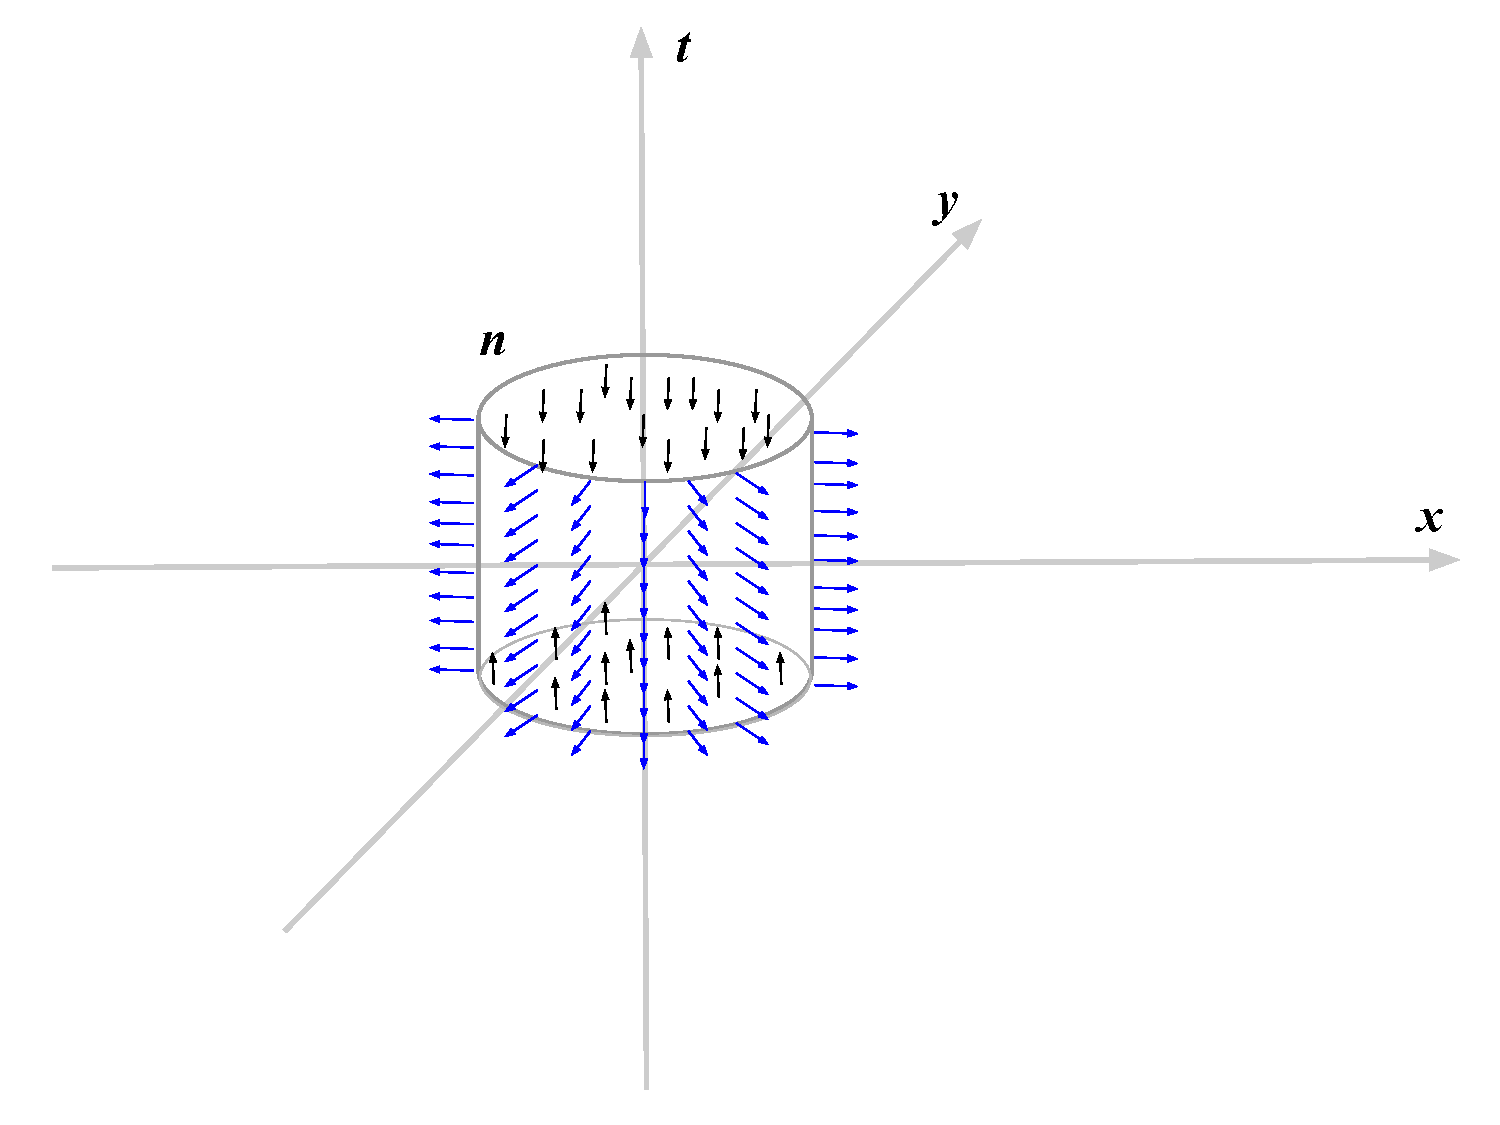
\includegraphics[scale=0.5]{figs/SpaceTimeNormal}
\caption{Normal vectors to the oriented surface in spacetime. Blue arrows indicate spacelike vectors. Black arrows indicate timelike vectors.}
\end{figure}

In the context of Special Theory of Relativity the equation \ref{divergence-theorem} becomes
\begin{equation}
\label{divergence-theorem-special}
\int_M \partial_\mu v^\mu d^4 x = \int_{\partial M} v^\mu dn_\mu.
\end{equation} 

\begin{theorem} (Relativistic Field Euler-Lagrange equations) If $${\delta} (S[\phi_0^\alpha, M]) = 0$$ for variation ${\delta}$ with all partial derivatives $\partial_\mu {\delta}\phi^\alpha$ and $\partial_\nu\partial_\mu \delta\phi^\alpha$ infinitesimal of the first order and ${\delta} \phi^\alpha$ vanishes on $\partial M$, then
\begin{equation} 
 \cfrac{\partial \mathcal{L}}{\partial \phi^\alpha} - \partial_\mu \Pi^\mu_\alpha = 0
\end{equation}
for $\phi_0^\alpha$ on the interior of $M$.
\end{theorem}   
\begin{proof}
Let $S = S[\phi_0^\alpha, M]$, then $\delta S = \int_M \delta \mathcal{L} d^4 x$. From (\ref{variation-lagrangian}) it follows that
\begin{equation}
{\delta} S = \int_M \bigg(\cfrac{\partial \mathcal{L}}{\partial \phi^\alpha} - \partial_\mu \Pi^\mu_\alpha \bigg){\delta}\phi^\alpha d^4 x + \int_M\partial_\mu(\Pi^\mu_\alpha {\delta}\phi^\alpha) d^4x.
\end{equation}
By Divergence Theorem (\ref{divergence-theorem-special}), we have
\begin{equation}
\int_M\partial_\mu(\Pi^\mu_\alpha {\delta}\phi^\alpha) d^4x = \int_{\partial M} \Pi^\mu_\alpha {\delta}\phi^\alpha dn_\mu = 0,
\end{equation}
because ${\delta} \phi^\alpha$ vanishes on $\partial M$. Then
\begin{equation}
{\delta} S = \int_M \bigg(\cfrac{\partial \mathcal{L}}{\partial \phi^\alpha} - \partial_\mu \Pi^\mu_\alpha \bigg){\delta}\phi^\alpha d^4 x.
\end{equation}
Since ${\delta} S = 0$ and ${\delta}\phi^\alpha$ is arbitrary enough, we have
\begin{equation}
\cfrac{\partial \mathcal{L}}{\partial \phi^\alpha} - \partial_\mu \Pi^\mu_\alpha = 0.
\end{equation}
\end{proof}

Consider an infinitesimal continuous symmetry $x \mapsto x + \hat{\delta} x$. From now on in this section, we will use $\hat{\delta}$ to denote an infinitesimal continuous symmetry variation. Note that in this section, we don't apply $\hat{\delta}$ as transformation of coordinates, we will use it only to shift the field relative to the frame of reference. We work all the time in an arbitrarily fixed frame of reference $x^\mu$ and we don't change it through out the whole chapter. This is why we don't need to transform Lagrangian density $\mathcal{L}$ and we use it all the time as exactly the same expression.

Let $\hat{\phi}^\alpha$ denote a field which was shifted in the direction $-\hat{\delta}x$ namely $\hat{\phi}^\alpha(x) = \phi^\alpha(x + \hat{\delta} x)$. Note that up to first order
\begin{equation}
\hat{\phi}^\alpha =  \phi^\alpha + \partial_\mu \phi^\alpha \hat{\delta} x^\mu,
\end{equation}
where $\hat{\delta} x^\mu = \hat{\delta} x^\mu(x)$ is a function of $x$ as in example (\ref{generator-symmetry}). We will use variation of $\phi^\alpha$ defined as $\hat{\delta} \phi^\alpha = \partial_\mu \phi^\alpha \hat{\delta} x^\mu$. Note that this variation moves the field in direction $-\hat{\delta} x$.

By $\hat{A}$ we will denote a set shifted in the direction $-\hat{\delta} x$.
\begin{equation}
\hat{A} = \{ x - \hat{\delta} x : x\in A \}.
\end{equation}
\begin{lemma}
\label{set_difference_noether}
If $F$ is an arbitrary continuous function on space-time then 
\begin{equation}
\int (\mathds{1}_{\hat{A}} - \mathds{1}_A)F d^4 x = \int\limits_{\partial A} F \hat{\delta} x^\mu dn_\mu.
\end{equation}
$n_\mu$ is understood as in (\ref{divergence-theorem-special}).
\end{lemma}
\begin{figure}[H]
\centering
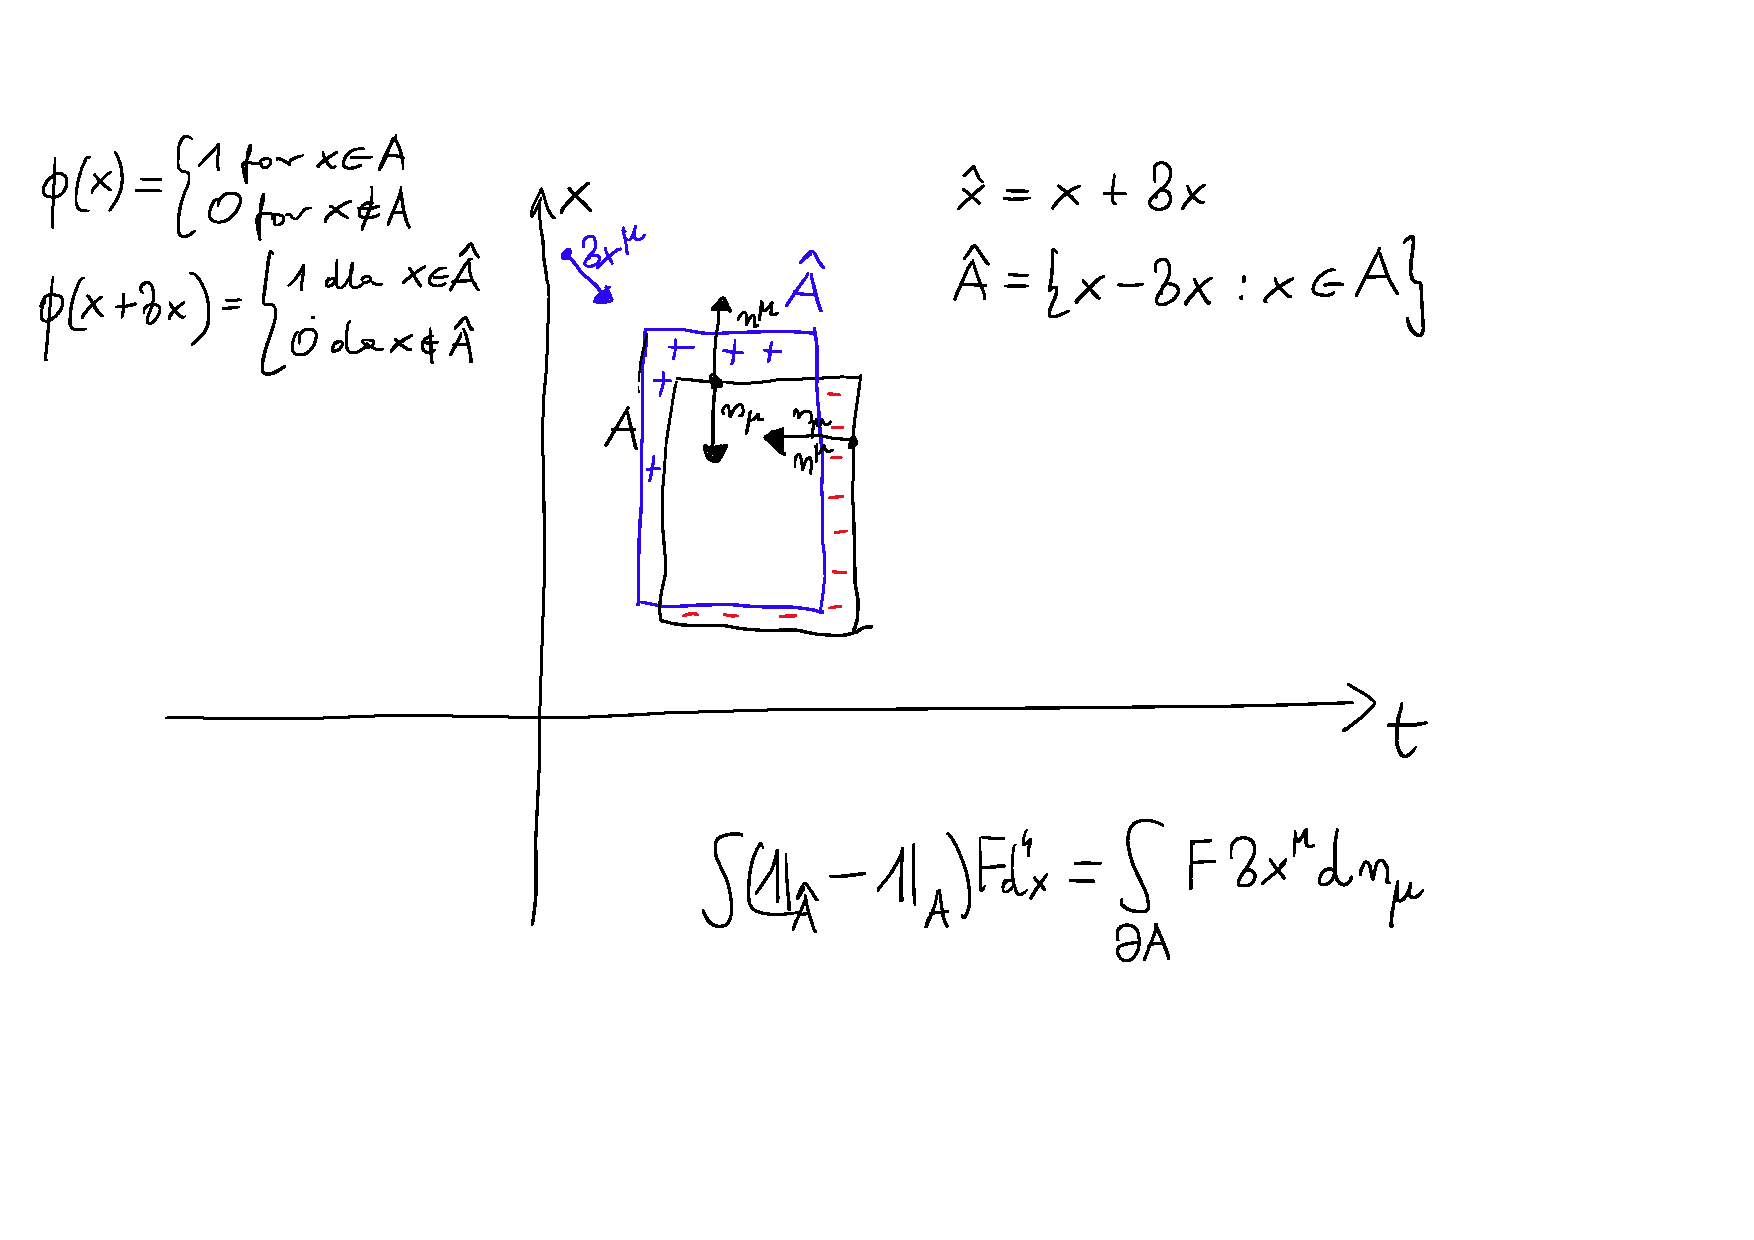
\includegraphics[scale=0.5]{figs/Noether1}
\caption{Illustration to visualise a proof of Lemma \ref{set_difference_noether}}
\end{figure}

Note that
\begin{equation}
\hat{\delta}S[\phi^\alpha, M] = S[\hat{\phi}^\alpha, \hat{M}] - S[\phi^\alpha, M]. 
\end{equation}

$\hat{\delta}S[\phi^\alpha, M]$ denotes difference in action when we move the field $\phi^\alpha$ by an infinitesimal continuous symmetry $-\hat{\delta} x$.

\begin{lemma}
\label{noether-variation}
If a field $\phi^\alpha$ is a stationary point of $S[ \cdot, M]$, then
\begin{equation}
\hat{\delta}S[\phi^\alpha, M] = \int\limits_M \partial_\mu \bigg( \Pi_\alpha^\mu \hat{\delta} \phi^\alpha + \hat{\delta}x^\mu \mathcal{L} \bigg)d^4 x.
\end{equation}
\end{lemma}
\begin{proof}
To make expressions shorter we will omit $(x)$ from $\phi^\alpha(x)$ and $\hat{\phi}^\alpha(x)$ when variable $x$ is obvious and we will write just $\mathcal{L}$ when applied to $(\phi^\alpha(x), \partial_\mu \phi^\alpha(x), x^\mu)$.
\begin{multline*}
\\
\hat{\delta}S[\phi^\alpha, M] = \int\limits_{\hat{M}} 
\mathcal{L}(\hat{\phi}^\alpha(x), \partial_\mu \hat{\phi}^\alpha(x), x^\mu) d^4 x -
\int\limits_M \mathcal{L}(\phi^\alpha(x), \partial_\mu \phi^\alpha(x), x^\mu) d^4 x
\\ = \int (\mathds{1}_{M} + \mathds{1}_{\hat{M}} - \mathds{1}_{M})
\mathcal{L}(\hat{\phi}^\alpha, \partial_\mu \hat{\phi}^\alpha, x^\mu) d^4 x
- \int\limits_M \mathcal{L}(\phi^\alpha, \partial_\mu \phi^\alpha, x^\mu) d^4 x
\\ = \int\limits_{M} 
\mathcal{L}(\hat{\phi}^\alpha(x), \partial_\mu \hat{\phi}^\alpha(x), x^\mu) d^4 x - \int\limits_M \mathcal{L}(\phi^\alpha, \partial_\mu \phi^\alpha, x^\mu) d^4 x
+ \int (\mathds{1}_{\hat{M}} - \mathds{1}_{M})
\mathcal{L}(\hat{\phi}^\alpha, \partial_\mu \hat{\phi}^\alpha, x^\mu) d^4 x
\\ =  \int\limits_{M} 
\mathcal{L}(\hat{\phi}^\alpha(x), \partial_\mu \hat{\phi}^\alpha(x), x^\mu) - \mathcal{L}(\phi^\alpha, \partial_\mu \phi^\alpha, x^\mu) d^4 x + 
\int (\mathds{1}_{\hat{M}} - \mathds{1}_{M})
(\mathcal{L} + \hat{\delta}\mathcal{L}) d^4 x
\\ = \int\limits_M \bigg(\cfrac{\partial \mathcal{L}}{\partial \phi^\alpha} - \partial_\mu \Pi^\mu_\alpha \bigg){\hat{\delta}}\phi^\alpha + \partial_\mu(\Pi^\mu_\alpha {\hat{\delta}}\phi^\alpha)d^4 x
+ \int\limits_{\partial M} (\mathcal{L} + \hat{\delta}\mathcal{L}) \hat{\delta} x^\mu dn_\mu
\\ = \int\limits_M \partial_\mu(\Pi^\mu_\alpha {\hat{\delta}}\phi^\alpha)d^4 x + \int\limits_{\partial M} \mathcal{L} \hat{\delta} x^\mu dn_\mu = \int\limits_M \partial_\mu(\Pi^\mu_\alpha {\hat{\delta}}\phi^\alpha)d^4 x + \int\limits_{\partial M} \partial_\mu (\mathcal{L} \hat{\delta} x^\mu) d^4 x
\\ =  \int\limits_M \partial_\mu \bigg( \Pi_\alpha^\mu \hat{\delta} \phi^\alpha + \hat{\delta}x^\mu \mathcal{L} \bigg)d^4 x.
\\
\end{multline*}

In transition from line 4 to 5 we used Lemma \ref{variation-lagrangian} and Lemma \ref{set_difference_noether} correspondingly. Calculations are done up to first order.

\end{proof}

For $\mathcal{L} = \mathcal{L}(\phi^\alpha, \partial_\mu \phi^\alpha, x^\mu)$ to have physical meaning one might require that if a field $\phi^\alpha$ is a stationary point of $S[\cdot, M]$, then the same field but shifted in space-time by an infinitesimal continuous symmetry $-\hat{\delta}x$ denoted as $\hat{\phi}^\alpha$ should be also a stationary point of $S[\cdot, \hat{M}]$. In other words, orientation of the field against arbitrary fixed frame of reference $x^\mu$ shouldn't matter. This is an assumption of isotropy and homogeneity of space.

In the next Lemma we will show that if $\hat{\delta} \mathcal{L} = \hat{\delta} \epsilon \partial_\mu f^\mu(\phi^\alpha, \partial_\mu \phi^\alpha, x)$ then $\mathcal{L}$ has these symmetry invariant stationary points in the above sense. In this context $\partial_\mu$ is a full derivative with respect to $x^\mu$. Note that a particular case of this is $\hat{\delta} \mathcal{L} = 0$.

\begin{lemma}
If $\hat{\delta} \mathcal{L} = \hat{\delta} \epsilon \partial_\mu f^\mu(\phi^\alpha, \partial_\mu \phi^\alpha, x^\mu)$ and a field $\phi_0^\alpha$ is a stationary point of $S[\cdot, M]$, then a field $\hat{\phi}_0^\alpha$ is a stationary point of $S[\cdot, \hat{M}]$.
\end{lemma}
\begin{proof}
Let's take an arbitrary field $\phi^\alpha$ not necessarily stationary.
We will show that
\begin{equation}
\label{noether-boudary}
S[\hat{\phi}^\alpha, \hat{M}] = S[\phi^\alpha, M] + \int\limits_{\partial M} \hat{\delta}\epsilon f^\mu(\phi^\alpha, \partial_\mu \phi^\alpha, x) + 
\mathcal{L}(\phi^\alpha, \partial_\mu \phi^\alpha, x^\mu)\hat{\delta}x^\mu dn_\mu.
\end{equation}

Indeed,
\begin{multline*}
\\
S[\hat{\phi}^\alpha, \hat{M}] = \int\limits_{\hat{M}}
\mathcal{L}(\hat{\phi}^\alpha, \partial_\mu \hat{\phi}^\alpha, x^\mu) d^4 x = \int\limits_{\hat{M}} \mathcal{L} + \hat{\delta} \mathcal{L} d^4 x
\\ = \int\limits_{M} \mathcal{L} + \hat{\delta} \mathcal{L} d^4 + \int (\mathds{1}_{\hat{M}} - \mathds{1}_{M})( \mathcal{L} + \hat{\delta} \mathcal{L}) d^4 x
\\ = S[\phi^\alpha, M] + \int\limits_M  \hat{\delta} \epsilon \partial_\mu f^\mu(\phi^\alpha, \partial_\mu \phi^\alpha, x^\mu) d^4x
+ \int\limits_{\partial M} (\mathcal{L} + \hat{\delta}\mathcal{L}) \hat{\delta} x^\mu dn_\mu
\\ = S[\phi^\alpha, M] + \int\limits_{\partial M} (\hat{\delta}\epsilon f^\mu(\phi^\alpha, \partial_\mu \phi^\alpha, x^\mu) + 
\mathcal{L}(\phi^\alpha, \partial_\mu \phi^\alpha, x^\mu)\hat{\delta}x^\mu) dn_\mu.
\\
\end{multline*}
Take any variation of the field $\delta \phi^\alpha$ for which $\delta \phi^\alpha = \partial_\mu \delta \phi^\alpha = 0$ on $\partial M$. Note that because $\delta \hat{\phi}^\alpha (x) = \delta \hat{\phi}^\alpha (x + \hat{\delta}x)$, we have  $\delta \hat{\phi}^\alpha = \partial_\mu \delta \hat{\phi}^\alpha = 0$ on $\partial \hat{M}$.

Since (\ref{noether-boudary}) was for an arbitrary field we have
\begin{multline*}
S[\hat{\phi}_0^\alpha + \delta \hat{\phi}^\alpha, \hat{M}] = S[\phi_0^\alpha + \delta \phi^\alpha, M] 
\\+ \int\limits_{\partial M} \bigg(\hat{\delta}\epsilon f^\mu(\phi_0^\alpha + \delta \phi^\alpha, \partial_\mu \phi_0^\alpha + \partial_\mu \delta \phi^\alpha, x^\mu) +  
\mathcal{L}(\phi_0^\alpha + \delta \phi^\alpha, \partial_\mu \phi_0^\alpha + \partial_\mu \delta \phi^\alpha, x^\mu)\hat{\delta}x^\mu\bigg) dn_\mu.
\end{multline*}
But since $\delta \phi^\alpha = \partial_\mu \delta \phi^\alpha = 0$ on $\partial M$, we have
\begin{multline*}
S[\hat{\phi}_0^\alpha + \delta \hat{\phi}^\alpha, \hat{M}] = S[\phi_0^\alpha + \delta \phi^\alpha, M] 
\\+ \int\limits_{\partial M} \bigg(\hat{\delta}\epsilon f^\mu(\phi_0^\alpha, \partial_\mu \phi_0^\alpha, x^\mu)  +
\mathcal{L}(\phi_0^\alpha, \partial_\mu \phi_0^\alpha, x^\mu)\hat{\delta}x^\mu\bigg) dn_\mu.
\end{multline*}
Hence,
\begin{equation}
S[\hat{\phi}_0^\alpha + \delta \hat{\phi}^\alpha, \hat{M}] = S[\phi_0^\alpha + \delta \phi^\alpha, M] + C(\phi_0^\alpha).
\end{equation}
and from that it follows that
a field $\hat{\phi}_0^\alpha$ is a stationary point of $S[\cdot, \hat{M}]$. 
\end{proof}

Now, we are ready to prove a celebrated Noether's theorem, in which one derives a locally conserved Noether's current $J^\mu$ from the invariance of stationary-point field under a chosen infinitesimal continuous symmetry of time-space for a given action functional.

\begin{theorem}(Noether's Theorem)
If $\hat{\delta} \mathcal{L} = \hat{\delta} \epsilon \partial_\mu f^\mu(\phi^\alpha, \partial_\mu \phi^\alpha, x)$ and a field $\phi_0^\alpha$ is a stationary point of $S[\cdot, M]$ for an arbitrary $M$, then for
\begin{equation}
J^\mu = \Pi_\alpha^\mu \partial_\nu \phi_0^\alpha \hat{\delta} x^\nu - \hat{\delta} \epsilon f^\mu,
\end{equation}
we have 
\begin{equation}
\partial_\mu J^\mu = 0.
\end{equation}
\end{theorem}
\begin{proof}
We will make all calculations for fixed $\phi^\alpha = \phi_0^\alpha$.
From Lemma \ref{noether-variation}, we have
\begin{equation}
\hat{\delta}S[\phi^\alpha, M] = \int\limits_M \partial_\mu \bigg( \Pi_\alpha^\mu \hat{\delta} \phi^\alpha + \hat{\delta}x^\mu \mathcal{L} \bigg)d^4 x.
\end{equation}
On the other hand from (\ref{noether-boudary}) we have
\begin{equation}
\hat{\delta}S[\phi^\alpha, M] = \int\limits_{M} \partial_\mu\bigg(\hat{\delta}\epsilon f^\mu(\phi^\alpha, \partial_\mu \phi^\alpha, x) + 
\mathcal{L}(\phi^\alpha, \partial_\mu \phi^\alpha, x^\mu)\hat{\delta}x^\mu\bigg)d^4 x.
\end{equation}
Thus
\begin{equation}
0 = \int\limits_{M} \partial_\mu \bigg( \Pi_\alpha^\mu \hat{\delta} \phi^\alpha - \hat{\delta}\epsilon f^\mu(\phi^\alpha, \partial_\mu \phi^\alpha, x)
\bigg)d^4 x.
\end{equation}
and since $M$ is arbitrary
\begin{equation}
\partial_\mu \bigg( \Pi_\alpha^\mu \hat{\delta} \phi^\alpha - \hat{\delta}\epsilon f^\mu(\phi^\alpha, \partial_\mu \phi^\alpha, x)
\bigg) = 0.
\end{equation}
From the above and because $\hat{\delta} \phi^\alpha = \partial_\mu \phi^\alpha \hat{\delta} x^\mu$, for
\begin{equation}
J^\mu = \Pi_\alpha^\mu \partial_\nu \phi^\alpha \hat{\delta} x^\nu - \hat{\delta} \epsilon f^\mu,
\end{equation}
we have $\partial_\mu J^\mu = 0$.
\end{proof}

\paragraph{Momentum preservation}
Let $\phi^\alpha$ be a field which is a stationary point of an action functional for certain Lagrangian density $\L$. Consider infinitesimal translation $\hat{\phi}^\alpha(x) = \phi^\alpha(x + \hat{\delta}\epsilon a)$ where $a$ is a constant $4$-vector.

Note that 
\begin{multline*}
\\
\hat{\delta} \mathcal{L} = \mathcal{L}(\phi^\alpha(x + \hat{\delta}\epsilon a), \partial_\mu \phi^\alpha(x + \hat{\delta}\epsilon a), x^\mu) -
\mathcal{L}(\phi^\alpha, \partial_\mu \phi^\alpha, x^\mu)
\\ = \hat{\delta}\epsilon \partial_\mu\L a^\mu = \hat{\delta}\epsilon \partial_\mu(\L a)^\mu.
\\
\end{multline*}

Mind that $\partial_\mu$ is a full derivative with respect to $x^\mu$. The locally conserved Noether's current for infinitesimal translation is then:
\begin{multline*}\\
J^\mu = \delta \epsilon(a^\nu \Pi_\alpha^\mu \partial_\nu \phi^\alpha - a^\mu\L)
\\ = \delta \epsilon a^\nu ( \Pi_\alpha^\mu \partial_\nu \phi^\alpha - \delta^\mu_\nu\L).
\\
\end{multline*}

If we consider translation along $x^0$ axis, let's assume $a = (1, 0, 0, 0)$, then 
\begin{equation}
J^0 = \delta\epsilon(\Pi_\alpha^0 \partial_0 \phi^\alpha - \L),
\end{equation}
which is related to energy conservation
and 
\begin{equation}
J^k = \delta \epsilon \Pi_\alpha^k \partial_k \phi^\alpha,
\end{equation}
which is related to momentum conservation along axis $x^k$.
  
\end{document}